% Options for packages loaded elsewhere
\PassOptionsToPackage{unicode}{hyperref}
\PassOptionsToPackage{hyphens}{url}
\PassOptionsToPackage{dvipsnames,svgnames,x11names}{xcolor}
%
\documentclass[
  letterpaper,
  DIV=11,
  numbers=noendperiod]{scrreprt}

\usepackage{amsmath,amssymb}
\usepackage{lmodern}
\usepackage{iftex}
\ifPDFTeX
  \usepackage[T1]{fontenc}
  \usepackage[utf8]{inputenc}
  \usepackage{textcomp} % provide euro and other symbols
\else % if luatex or xetex
  \usepackage{unicode-math}
  \defaultfontfeatures{Scale=MatchLowercase}
  \defaultfontfeatures[\rmfamily]{Ligatures=TeX,Scale=1}
\fi
% Use upquote if available, for straight quotes in verbatim environments
\IfFileExists{upquote.sty}{\usepackage{upquote}}{}
\IfFileExists{microtype.sty}{% use microtype if available
  \usepackage[]{microtype}
  \UseMicrotypeSet[protrusion]{basicmath} % disable protrusion for tt fonts
}{}
\makeatletter
\@ifundefined{KOMAClassName}{% if non-KOMA class
  \IfFileExists{parskip.sty}{%
    \usepackage{parskip}
  }{% else
    \setlength{\parindent}{0pt}
    \setlength{\parskip}{6pt plus 2pt minus 1pt}}
}{% if KOMA class
  \KOMAoptions{parskip=half}}
\makeatother
\usepackage{xcolor}
\setlength{\emergencystretch}{3em} % prevent overfull lines
\setcounter{secnumdepth}{5}
% Make \paragraph and \subparagraph free-standing
\ifx\paragraph\undefined\else
  \let\oldparagraph\paragraph
  \renewcommand{\paragraph}[1]{\oldparagraph{#1}\mbox{}}
\fi
\ifx\subparagraph\undefined\else
  \let\oldsubparagraph\subparagraph
  \renewcommand{\subparagraph}[1]{\oldsubparagraph{#1}\mbox{}}
\fi


\providecommand{\tightlist}{%
  \setlength{\itemsep}{0pt}\setlength{\parskip}{0pt}}\usepackage{longtable,booktabs,array}
\usepackage{calc} % for calculating minipage widths
% Correct order of tables after \paragraph or \subparagraph
\usepackage{etoolbox}
\makeatletter
\patchcmd\longtable{\par}{\if@noskipsec\mbox{}\fi\par}{}{}
\makeatother
% Allow footnotes in longtable head/foot
\IfFileExists{footnotehyper.sty}{\usepackage{footnotehyper}}{\usepackage{footnote}}
\makesavenoteenv{longtable}
\usepackage{graphicx}
\makeatletter
\def\maxwidth{\ifdim\Gin@nat@width>\linewidth\linewidth\else\Gin@nat@width\fi}
\def\maxheight{\ifdim\Gin@nat@height>\textheight\textheight\else\Gin@nat@height\fi}
\makeatother
% Scale images if necessary, so that they will not overflow the page
% margins by default, and it is still possible to overwrite the defaults
% using explicit options in \includegraphics[width, height, ...]{}
\setkeys{Gin}{width=\maxwidth,height=\maxheight,keepaspectratio}
% Set default figure placement to htbp
\makeatletter
\def\fps@figure{htbp}
\makeatother
\newlength{\cslhangindent}
\setlength{\cslhangindent}{1.5em}
\newlength{\csllabelwidth}
\setlength{\csllabelwidth}{3em}
\newlength{\cslentryspacingunit} % times entry-spacing
\setlength{\cslentryspacingunit}{\parskip}
\newenvironment{CSLReferences}[2] % #1 hanging-ident, #2 entry spacing
 {% don't indent paragraphs
  \setlength{\parindent}{0pt}
  % turn on hanging indent if param 1 is 1
  \ifodd #1
  \let\oldpar\par
  \def\par{\hangindent=\cslhangindent\oldpar}
  \fi
  % set entry spacing
  \setlength{\parskip}{#2\cslentryspacingunit}
 }%
 {}
\usepackage{calc}
\newcommand{\CSLBlock}[1]{#1\hfill\break}
\newcommand{\CSLLeftMargin}[1]{\parbox[t]{\csllabelwidth}{#1}}
\newcommand{\CSLRightInline}[1]{\parbox[t]{\linewidth - \csllabelwidth}{#1}\break}
\newcommand{\CSLIndent}[1]{\hspace{\cslhangindent}#1}

\KOMAoption{captions}{tableheading}
\makeatletter
\makeatother
\makeatletter
\@ifpackageloaded{bookmark}{}{\usepackage{bookmark}}
\makeatother
\makeatletter
\@ifpackageloaded{caption}{}{\usepackage{caption}}
\AtBeginDocument{%
\ifdefined\contentsname
  \renewcommand*\contentsname{Table of contents}
\else
  \newcommand\contentsname{Table of contents}
\fi
\ifdefined\listfigurename
  \renewcommand*\listfigurename{List of Figures}
\else
  \newcommand\listfigurename{List of Figures}
\fi
\ifdefined\listtablename
  \renewcommand*\listtablename{List of Tables}
\else
  \newcommand\listtablename{List of Tables}
\fi
\ifdefined\figurename
  \renewcommand*\figurename{Figure}
\else
  \newcommand\figurename{Figure}
\fi
\ifdefined\tablename
  \renewcommand*\tablename{Table}
\else
  \newcommand\tablename{Table}
\fi
}
\@ifpackageloaded{float}{}{\usepackage{float}}
\floatstyle{ruled}
\@ifundefined{c@chapter}{\newfloat{codelisting}{h}{lop}}{\newfloat{codelisting}{h}{lop}[chapter]}
\floatname{codelisting}{Listing}
\newcommand*\listoflistings{\listof{codelisting}{List of Listings}}
\makeatother
\makeatletter
\@ifpackageloaded{caption}{}{\usepackage{caption}}
\@ifpackageloaded{subcaption}{}{\usepackage{subcaption}}
\makeatother
\makeatletter
\@ifpackageloaded{tcolorbox}{}{\usepackage[many]{tcolorbox}}
\makeatother
\makeatletter
\@ifundefined{shadecolor}{\definecolor{shadecolor}{rgb}{.97, .97, .97}}
\makeatother
\makeatletter
\makeatother
\ifLuaTeX
  \usepackage{selnolig}  % disable illegal ligatures
\fi
\IfFileExists{bookmark.sty}{\usepackage{bookmark}}{\usepackage{hyperref}}
\IfFileExists{xurl.sty}{\usepackage{xurl}}{} % add URL line breaks if available
\urlstyle{same} % disable monospaced font for URLs
\hypersetup{
  pdftitle={Big Data Programming for Data Scientists},
  pdfauthor={J. Hathaway},
  colorlinks=true,
  linkcolor={blue},
  filecolor={Maroon},
  citecolor={Blue},
  urlcolor={Blue},
  pdfcreator={LaTeX via pandoc}}

\title{Big Data Programming for Data Scientists}
\author{J. Hathaway}
\date{1/12/23}

\begin{document}
\maketitle
\ifdefined\Shaded\renewenvironment{Shaded}{\begin{tcolorbox}[sharp corners, breakable, interior hidden, enhanced, borderline west={3pt}{0pt}{shadecolor}, frame hidden, boxrule=0pt]}{\end{tcolorbox}}\fi

\renewcommand*\contentsname{Table of contents}
{
\hypersetup{linkcolor=}
\setcounter{tocdepth}{2}
\tableofcontents
}
\bookmarksetup{startatroot}

\hypertarget{preface}{%
\chapter*{Preface}\label{preface}}
\addcontentsline{toc}{chapter}{Preface}

\markboth{Preface}{Preface}

This is a Quarto book.

To learn more about Quarto books visit
\url{https://quarto.org/docs/books}.

\bookmarksetup{startatroot}

\hypertarget{introduction}{%
\chapter{Introduction}\label{introduction}}

\hypertarget{using-spark-for-exploratory-data-analysis}{%
\section{Using Spark for exploratory data
analysis}\label{using-spark-for-exploratory-data-analysis}}

\hypertarget{what-is-spark}{%
\subsection{What is Spark?}\label{what-is-spark}}

\begin{quote}
From its humble beginnings in the AMPLab at U.C. Berkeley in 2009,
Apache Spark has become one of the key big data distributed processing
frameworks in the world. Spark can be deployed in various ways, provides
native bindings for the Java, Scala, Python, and R programming
languages, and supports SQL, streaming data, machine learning, and graph
processing. You'll find it used by banks, telecommunications companies,
games companies, governments, and all major tech giants such as Apple,
Facebook, IBM, and Microsoft.
\href{https://www.infoworld.com/article/3236869/what-is-apache-spark-the-big-data-platform-that-crushed-hadoop.html}{ref}
\end{quote}

Databricks provides \href{https://databricks.com/spark/about}{an
excellent overview} as well.

\hypertarget{rules-of-thumb-for-spark}{%
\subsection{Rules of thumb for Spark}\label{rules-of-thumb-for-spark}}

We are learning to use Spark as Data Scientists or Analysts that need
tools for exploring and analyzing data that pushes the boundaries of our
local memory. As we explore this space, we will need to keep in mind a
few \href{https://en.wikipedia.org/wiki/Rule_of_thumb}{rules of thumb}
that should guide our use of Spark.

\hypertarget{the-spark-apis-let-you-use-your-language-of-preference}{%
\subsubsection{The Spark APIs let you use your language of
preference}\label{the-spark-apis-let-you-use-your-language-of-preference}}

You can use Java, Scala, Python, or R to access Spark. Like
\href{https://en.wikipedia.org/wiki/Goldilocks_principle}{Goldilocks and
the Three Bears}, we want the language that is not `too hot' or `too
cold' for data science use. Java is a bit too verbose for day-to-day
data science work. Scala is fast but still a little verbose. Python is a
little slower but ingrained in the data science community, and R is less
easy to implement in a production environment.

\begin{itemize}
\tightlist
\item
  \textbf{pyspark (just right)}: The
  \href{https://spark.apache.org/docs/latest/api/python/index.html}{pyspark
  package} looks to be the `just the right amount' of the Spark APIs.\\
\item
  \textbf{sparkR (a little cold)}:
  \href{https://spark.apache.org/docs/latest/sparkr.html}{Apache has
  developed an R package} that is the official R connection to Spark.
\item
  \textbf{sparklyr (RStudio's warm-up)}: If you are experienced with the
  \href{https://www.tidyverse.org/}{Tidyverse}, then
  \href{https://spark.rstudio.com/}{RStudio's sparklyr} could pull you
  away from pyspark.
\end{itemize}

You can read a comparison of sparkR and sparklyr
\href{https://developpaper.com/deep-comparative-data-science-toolbox-sparkr-vs-sparklyr/}{here}.

\hypertarget{use-dataframes-ignore-rdds}{%
\subsubsection{Use DataFrames (ignore
RDDs)}\label{use-dataframes-ignore-rdds}}

For day-to-day data science use, \texttt{DataFrame}s are the option you
should choose.

\begin{enumerate}
\def\labelenumi{\arabic{enumi}.}
\tightlist
\item
  Spark has built a framework to optimize Resilient Distributed Dataset
  (RDD) use when we program with \texttt{DataFrame} methods.
\item
  Spark internally stores \texttt{DataFrame}s in a binary format, so
  there is no need to serialize and deserialize data as it moves over
  the cluster.
\end{enumerate}

Databricks provides a
\href{https://databricks.com/blog/2015/04/13/deep-dive-into-spark-sqls-catalyst-optimizer.html}{Deep
Dive into Spark SQL's Catalyst Optimizer} and
\href{https://databricks.com/blog/2016/07/14/a-tale-of-three-apache-spark-apis-rdds-dataframes-and-datasets.html}{A
Tale of Three Apache Spark APIs: RDDs vs.~DataFrames and Datasets} to
help you understand more depth on the relationship between
\texttt{DataFrame}s.

We pulled the bullets and image below from the Databricks articles.

\begin{quote}
\begin{itemize}
\tightlist
\item
  If you want unification and simplification of APIs across Spark
  Libraries, use DataFrame or Dataset.
\item
  If you are an R user, use DataFrames.
\item
  If you are a Python user, use DataFrames and resort back to RDDs if
  you need more control.
\end{itemize}
\end{quote}

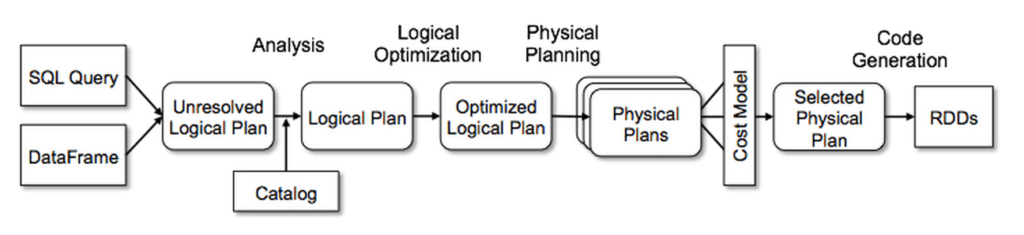
\includegraphics{./img/spark_sql_dataframe_rdd.png}

\hypertarget{write-and-read-serialized-data-formats}{%
\subsubsection{Write and Read serialized data
formats}\label{write-and-read-serialized-data-formats}}

The \href{https://databricks.com/glossary/what-is-parquet}{Apache
Parquet} format is optimal for most data science applications. It is a
serialized columnar format that provides speed and size benefits for big
data applications. The following table compares the savings and the
speedup obtained by converting data into Parquet from CSV.

\begin{longtable}[]{@{}
  >{\raggedright\arraybackslash}p{(\columnwidth - 8\tabcolsep) * \real{0.3243}}
  >{\raggedright\arraybackslash}p{(\columnwidth - 8\tabcolsep) * \real{0.2432}}
  >{\raggedright\arraybackslash}p{(\columnwidth - 8\tabcolsep) * \real{0.1261}}
  >{\raggedright\arraybackslash}p{(\columnwidth - 8\tabcolsep) * \real{0.1892}}
  >{\raggedright\arraybackslash}p{(\columnwidth - 8\tabcolsep) * \real{0.1171}}@{}}
\toprule()
\begin{minipage}[b]{\linewidth}\raggedright
Dataset
\end{minipage} & \begin{minipage}[b]{\linewidth}\raggedright
Size on Amazon S3
\end{minipage} & \begin{minipage}[b]{\linewidth}\raggedright
Query Run Time
\end{minipage} & \begin{minipage}[b]{\linewidth}\raggedright
Data Scanned
\end{minipage} & \begin{minipage}[b]{\linewidth}\raggedright
Cost
\end{minipage} \\
\midrule()
\endhead
Data stored as CSV files & 1 TB & 236 seconds & 1.15 TB & \$5.75 \\
Data stored in Apache Parquet Format & 130 GB & 6.78 seconds & 2.51 GB &
\$0.01 \\
Savings & 87\% less when using Parquet & 34x faster & 99\% less data
scanned & 99.7\% savings \\
\bottomrule()
\end{longtable}

You could use
\href{https://spark.apache.org/docs/latest/sql-data-sources-avro.html}{Avro
with Spark} as well. It is stored in rows, much like a \texttt{.csv}
file, but is serialized.

\hypertarget{databricks}{%
\section{DataBricks}\label{databricks}}

\hypertarget{navigation}{%
\subsection{Navigation}\label{navigation}}

\begin{itemize}
\tightlist
\item
  This file provides a high-level overview of Databricks.
\item
  The HTML folder contains notebooks that can be imported into
  Databricks. All HTML files in that folder can be imported
  individually, or you can use \texttt{examples.dbc} to import them all
  at once.
\end{itemize}

\hypertarget{the-elevator-pitches}{%
\subsection{The elevator pitches}\label{the-elevator-pitches}}

\emph{Check out these branded videos.}

\begin{quote}
\href{https://youtu.be/_1QQHv7T9og}{It's time for DataBricks!}
\end{quote}

\begin{quote}
\href{https://youtu.be/1cJ0XYaARBY}{Databricks is the AI Company}
\end{quote}

\emph{Here is a bit more nerdy DS/CS pitch
\href{https://databricks.com/company/about-us}{from their website}}

\begin{quote}
With origins in academia and the open-source community, Databricks was
founded in 2013 by the original creators of Apache Spark™, Delta Lake,
and MLflow. As the world's first and only lakehouse platform in the
cloud, Databricks combines the best of data warehouses and data lakes to
offer an open and unified platform for data and AI.
\end{quote}

\begin{quote}
\href{https://youtu.be/n-yt_3HvkOI}{Introduction to Databricks Unified
Data Platform: 5 min demo}
\end{quote}

\hypertarget{databricks-community-edition}{%
\subsection{Databricks Community
Edition}\label{databricks-community-edition}}

The \href{https://community.cloud.databricks.com/login.html}{community
edition} provides free access to the Databricks environment to see their
vision of jupyter notebooks and to work with a Spark environment. The
users do not incur any costs while using Databricks.

Read more about the limitations of Community Edition at
\href{https://databricks.com/product/faq/community-edition}{this FAQ}.

\hypertarget{community-edition-setup}{%
\subsubsection{Community Edition Setup}\label{community-edition-setup}}

\begin{enumerate}
\def\labelenumi{\arabic{enumi}.}
\tightlist
\item
  Create a \href{https://databricks.com/try-databricks}{community
  account on Databricks}
\item
  Login into the
  \href{https://community.cloud.databricks.com/login.html}{Databricks
  community edition portal}
\item
  Click the compute icon on the left
  (
\includegraphics{https://github.com/byuibigdata/project_safegraph/blob/main/img/compute_icon.png})
\item
  Name your cluster
\item
  Create your cluster and then navigate to the libraries tab to install
  our needed Python packages (for example \texttt{gql},
  \texttt{plotnine}, \texttt{altair}). Pandas is already installed.
\end{enumerate}

\hypertarget{what-is-the-difference-between-the-databricks-community-edition-and-the-full-databricks-platform}{%
\subsection{What is the difference between the Databricks Community
Edition and the full Databricks
Platform?}\label{what-is-the-difference-between-the-databricks-community-edition-and-the-full-databricks-platform}}

\begin{quote}
With the Databricks Community Edition, the users will have access to
15GB clusters, a cluster manager and the notebook environment to
prototype simple applications, and JDBC / ODBC integrations for BI
analysis. The Databricks Community Edition access is not time-limited
and users will not incur AWS costs for their cluster usage.
\end{quote}

\begin{quote}
The full Databricks platform offers production-grade functionality, such
as an unlimited number of clusters that easily scale up or down, a job
launcher, collaboration, advanced security controls, and expert support.
It helps users process data at scale, or build Apache Spark applications
in a team setting.
\end{quote}

\begin{quote}
\href{https://databricks.com/product/faq/community-edition}{Databricks}
\end{quote}

\hypertarget{using-databricks-notebooks}{%
\subsection{Using Databricks
notebooks}\label{using-databricks-notebooks}}

\begin{itemize}
\tightlist
\item
  \href{https://youtu.be/n-yt_3HvkOI}{Watch this video to see a short
  example of using the platform}
\item
  \href{https://subscription.packtpub.com/book/data/9781838647216/2/ch02lvl1sec08/using-azure-databricks-notebooks}{Read
  about the basics of Databricks notebooks}
\end{itemize}

\hypertarget{key-links}{%
\subsection{Key links}\label{key-links}}

\begin{itemize}
\tightlist
\item
  \href{https://databricks.com/try-databricks}{Sign up for Community
  Edition}
\item
  \href{https://towardsdatascience.com/databricks-notebooks-a-love-hate-relationship-8f73e5b291fb}{A
  love-hate relationship with Databricks Notebooks}
\item
  \href{https://subscription.packtpub.com/book/data/9781838647216/2/ch02lvl1sec08/using-azure-databricks-notebooks}{Databricks
  notebooks}
\item
  \href{https://youtu.be/ThrmPaleEiI}{Databricks Backstory}
\end{itemize}

\bookmarksetup{startatroot}

\hypertarget{references}{%
\chapter*{References}\label{references}}
\addcontentsline{toc}{chapter}{References}

\markboth{References}{References}

\hypertarget{refs}{}
\begin{CSLReferences}{0}{0}
\end{CSLReferences}



\end{document}
